\documentclass[13pt, t]{beamer}
% Presento style file
\usepackage{config/presento}

% custom command and packages
% custom packages
\usepackage{textpos}
\setlength{\TPHorizModule}{1cm}
\setlength{\TPVertModule}{1cm}

\newcommand\crule[1][black]{\textcolor{#1}{\rule{2cm}{2cm}}}



\usepackage{color, colortbl}

\title{\Large \hspace{-0.5cm} Analysing phonological systems: \\ on Bayesian typological research}
\author[shortname]{George Moroz}
\institute[shortinst]{Linguistic Convergence Laboratory, NRU HSE, Moscow, Russia}
\date{\begin{center} 24 August 2019 \bigskip \\ Societas Linguistica Europaea, 52nd Annual Meeting, Leipzig University\\ \vfill Presentation is available here: {\large \href{https://tinyurl.com/y3wtkcbq}{tinyurl.com/y3wtkcbq} \hfill 
\includegraphics[height = 2.5cm]{images/01_qrcode}} \end{center}}

\begin{document}

\begin{frame}[plain]
\maketitle
\end{frame}

\begin{frame}{In this talk I will cover the following:}
\begin{itemize}
\item Goals of linguistic typology
\item Different strategies of sampling
\item The Bayesian way of thinking about linguistic typology
\item Case study: vowels
\end{itemize}
\end{frame}

\begin{frame}{Goals of linguistic typology}
\begin{itemize}
\item Attest distributions (statistical and areal) of typological values \pause
\item Find a correlation between the distributions of different typological categories
\begin{itemize}
\item Absolute universals
\item Distributional patterns and tendencies
\item Semantic maps
\item Diachronic change of typological values \pause
\end{itemize}
\item Find a correlation between linguistic and non-linguistic patterns
\begin{itemize}
\item Population movements
\item Population size
\item Language contact
\item Sociolinguistic parameters
\item Geopolitical environment (including the spread of diseases) \pause
\end{itemize}
\item Deal with mixed typological values
\end{itemize}
\end{frame}

\begin{frame}{Frequentist typological research}
\begin{itemize}
\item Formulate a theoretical problem\\ % theoretical problem ili research question
There is a category in some languages with values \textbf{VAL 1} and \textbf{VAL 2}. \pause \\
What is the probability $\theta$ of finding \textbf{VAL 1} in a randomly picked language? \pause
\item[◌] Get a grant, hire some students, or select a holiday you want to spend working on this topic... \pause
\item Pick a sample of languages, calculate the desired statistics, e. g. $\hat{\theta}$ \pause
\item From now on $\hat{\theta}$ is the best estimation of $\theta$ that you know\pause, add some \textbf{confidence intervals} of you need to convince an editor who is mad about statistics
\item[◌] After you published your paper project is finished
\end{itemize}
\end{frame}

\begin{frame}{There are different type of sampling}
\begin{multicols}{2}
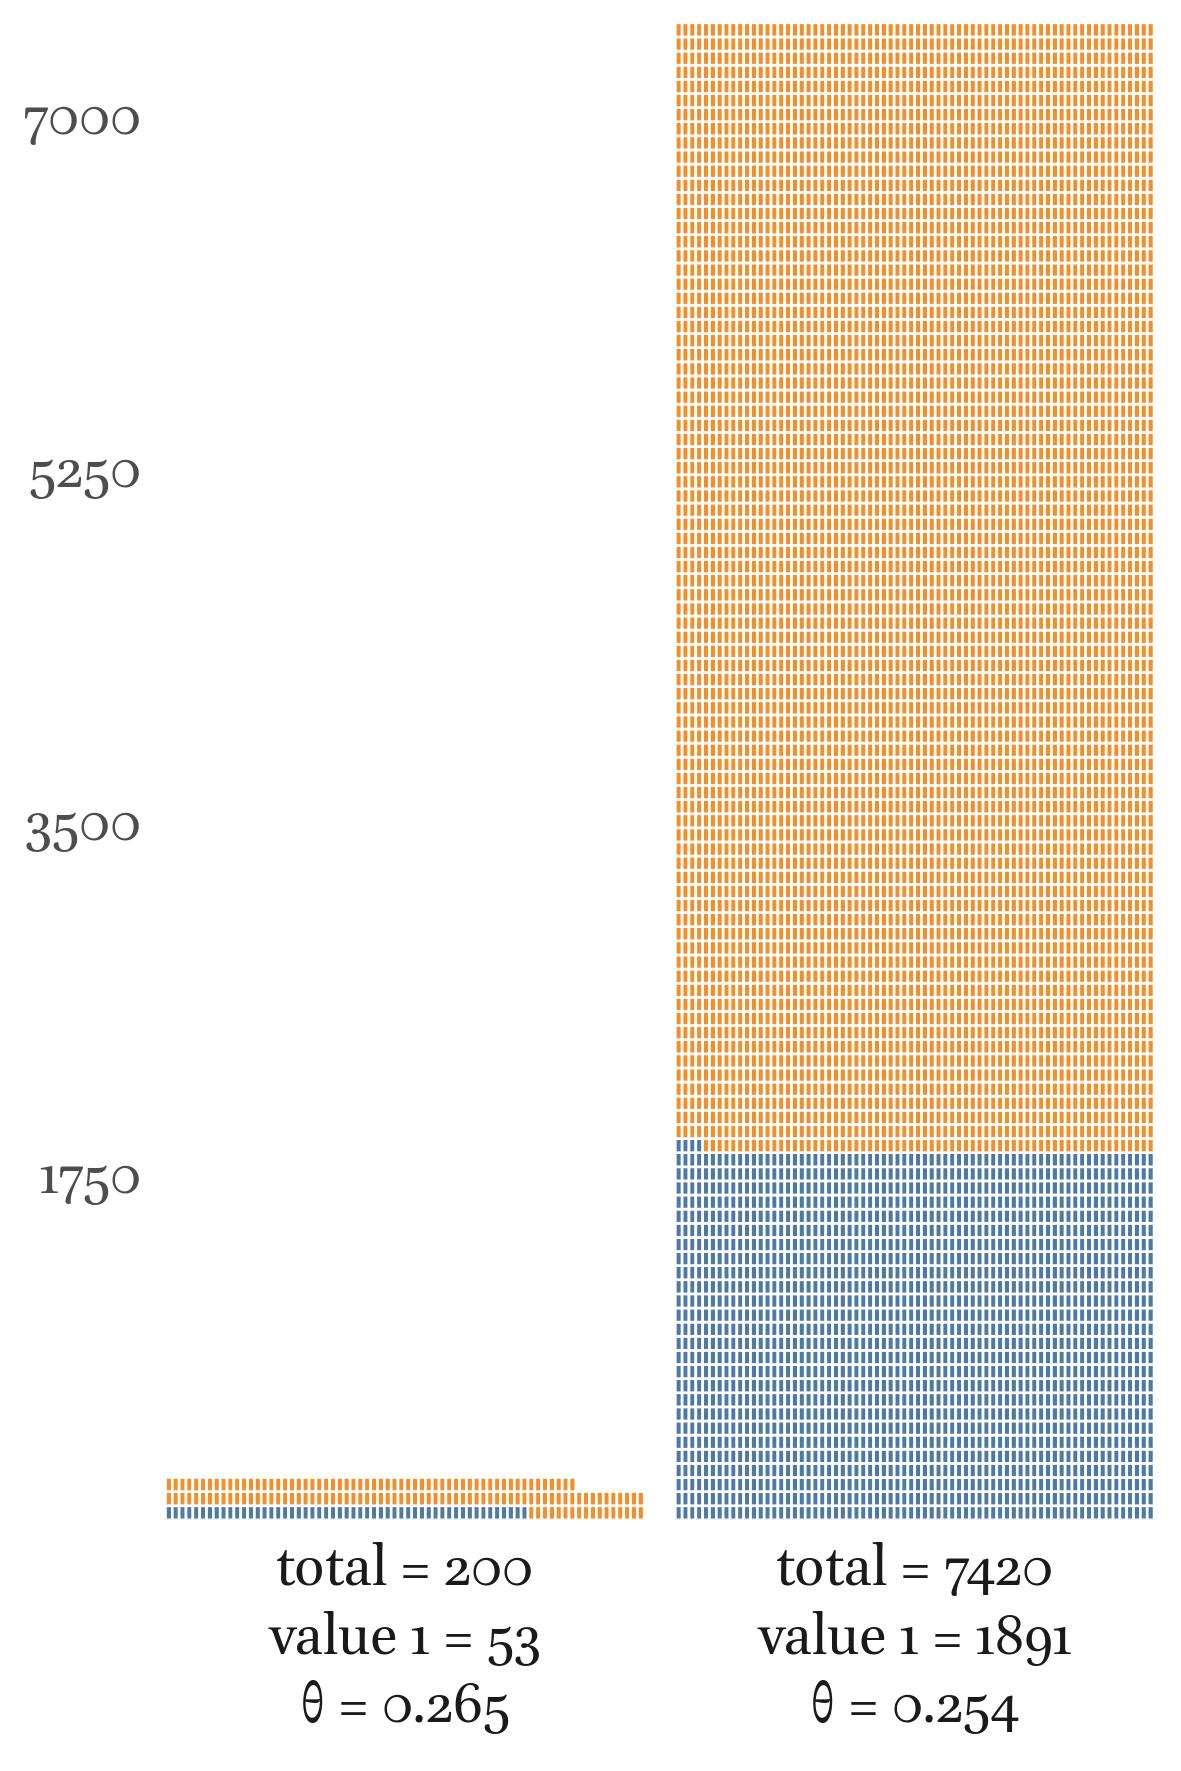
\includegraphics[width=\linewidth]{images/03_simple_sample}
\columnbreak

\textbf{Random sampling}\\
each member of the population has an equal probability of selection \pause\\
\begin{itemize}
\item[\color{colorblue}!!!] but each language is grouped in \textbf{a language family} and \textbf{an area}, so observations are not independent\dots
\end{itemize}

\end{multicols}
\end{frame}

\begin{frame}{Language families (languages > 10)}
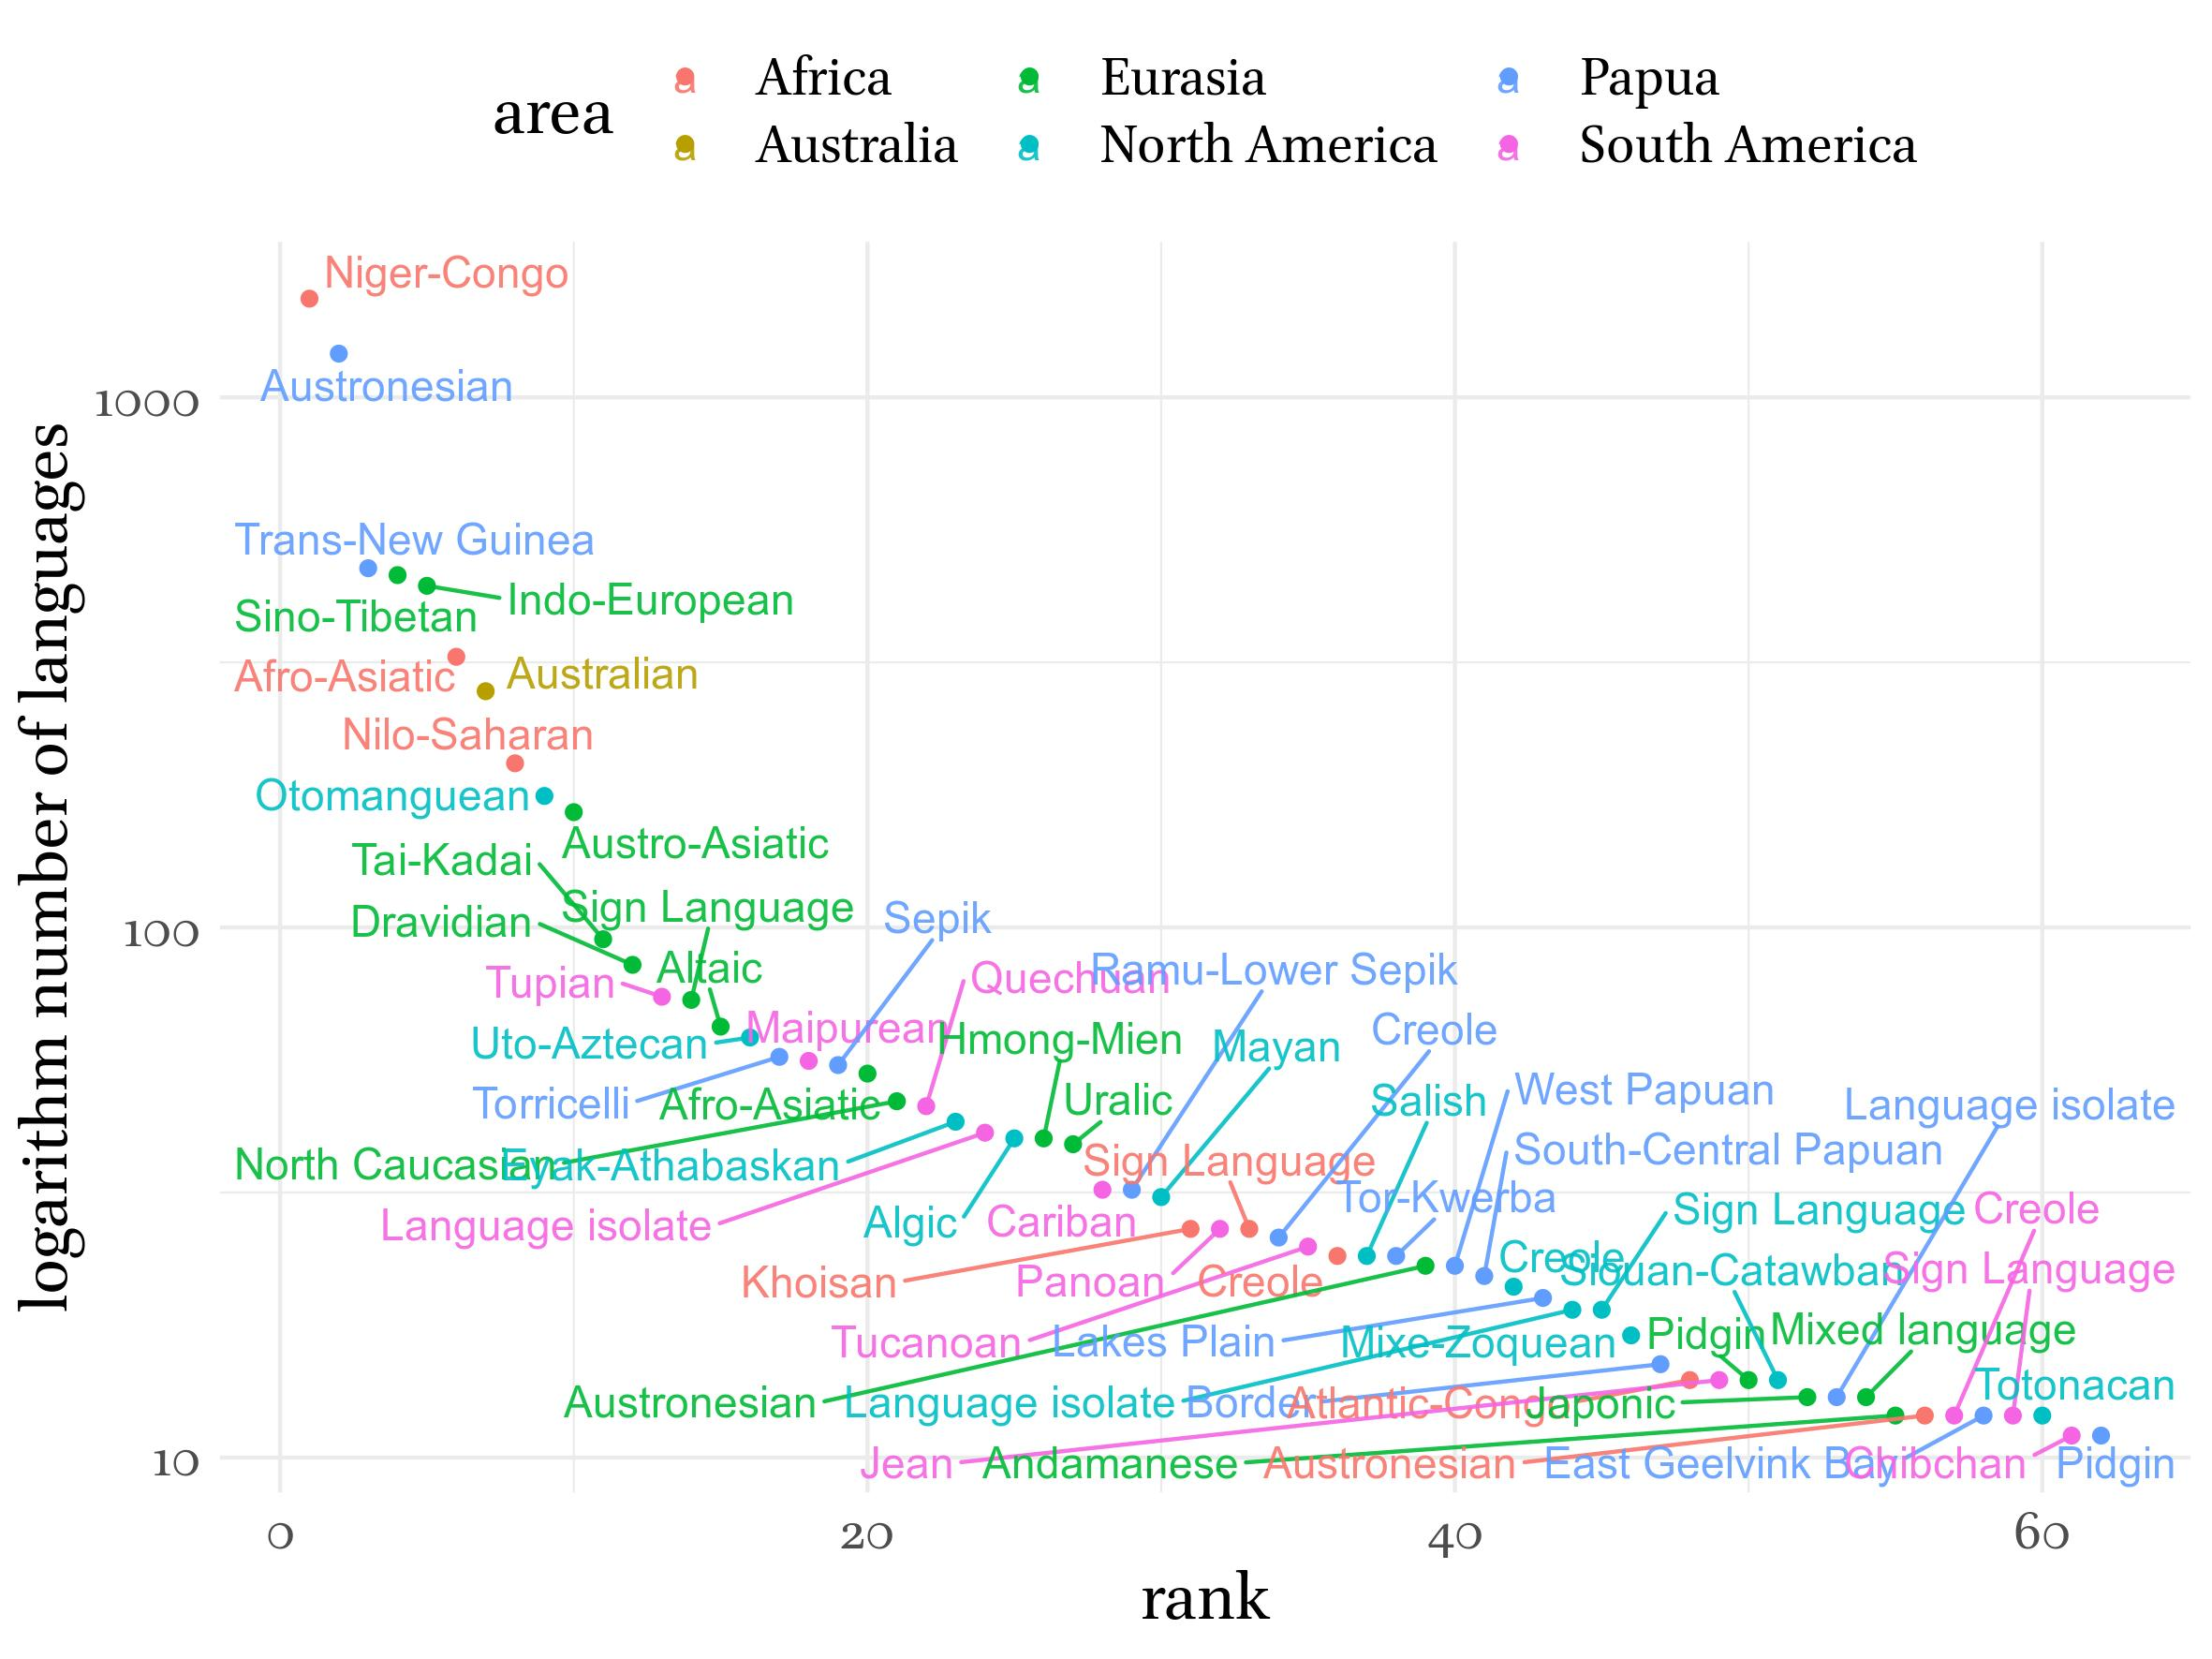
\includegraphics[width=\linewidth]{images/04_families_by_area}
\end{frame}

\begin{frame}{There are different type of sampling:}
\begin{multicols}{2}
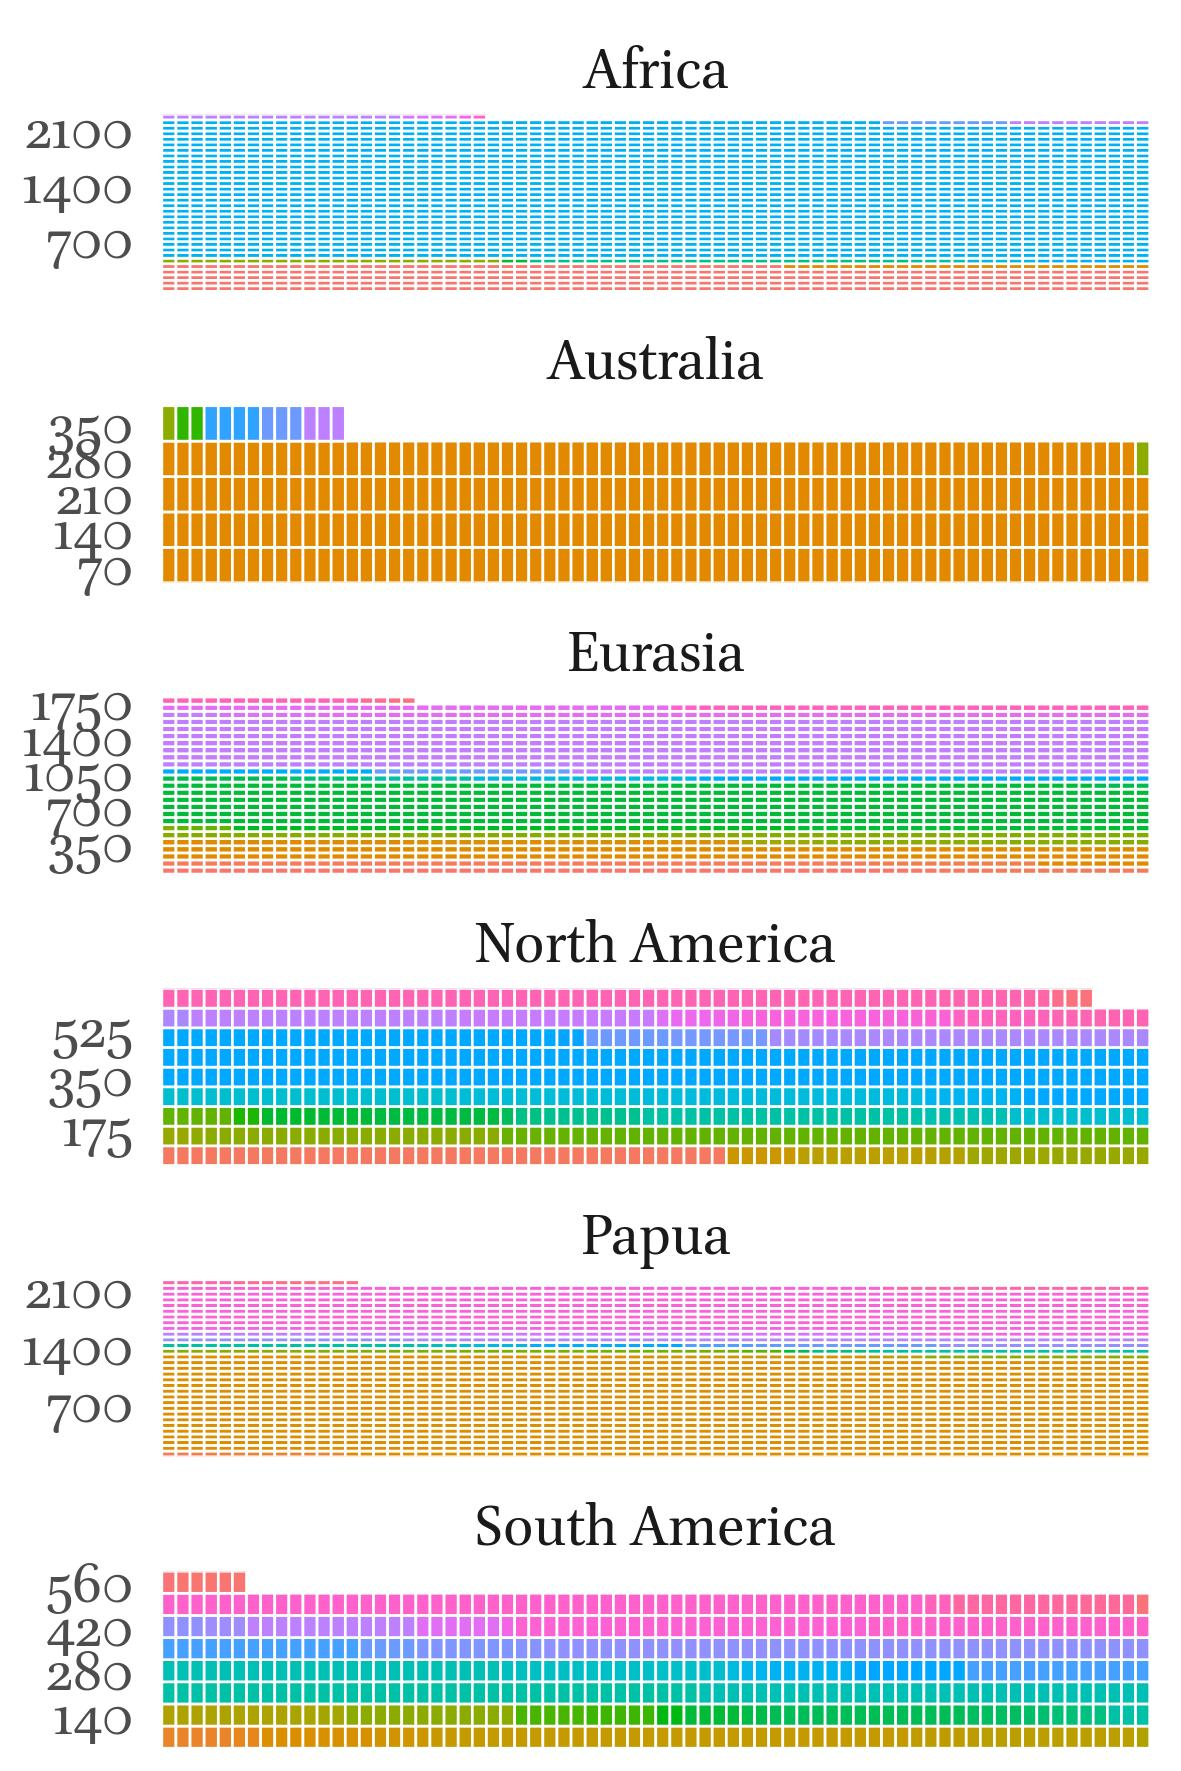
\includegraphics[width=\linewidth]{images/05_families_by_area}
\columnbreak

\textbf{Stratified random sampling}\\
divide the population into groups that differ in important ways, and then perform random sampling for each group\pause\\
\begin{itemize}
\item[\color{colorblue}!!!] The Glottolog version in the \texttt{\small lingtypology} package suggests that there are \\ \alert{214 unique combinations} (142 sign languages and 82 isolates counted as one family) % я бы добавила ссылку на версию глоттолога
\pause
\item[\color{colorblue}$\Rightarrow$] So to create a statistically reasonable sample one needs to get around 300 languages
\end{itemize}
\end{multicols}
\end{frame}

\begin{frame}{I am not the first to discuss this problem}
\begin{itemize}
\item \citep{bell78} "Language Samples"
\item \citep{dryer89} "Large Linguistic Areas and Language Sampling"
\item \citep{perkins89} "Statistical Techniques for Determining Language Sample Size"
\item \citep{nichols92} "Linguistic Diversity in Space and Time"
\item \citep{rietveld93} "Statistical Techniques for the Study of Language and Language Behaviour"
\item \citep{rijkhoff98} "Language sampling"
\item \citep{maslova00} "A dynamic approach to the verification of distributional universals"
\item \citep{widmann01} "Language Sampling for Typological Studies"
\item \citep{janssen06} "Randomization Tests in Language Typology"
\item \citep{bakker10} "Language Sampling"
\end{itemize}
\end{frame}

\begin{frame}{Biases of sampling}
\begin{itemize}
\item geneological
\item caused by contacts
\item cultural
\item typological
\item populational \pause
\item \Large \alert{bibliographical} \pause
\item \LARGE \alert{typologistical} --- because only typologists think that there is only one typological value per one so called language
\end{itemize}
\end{frame}

\begin{frame}
\begin{multicols}{2}
``theoretical linguists''
\begin{itemize}
\item complain about how hard is to solve a problem
\item don't publish any results, until it will be ideal
\end{itemize}
\columnbreak
``computational linguists''
\begin{itemize}
\item solve the wrong problem
\item publish a messy results
\end{itemize}
\vfill
\ \pause
\end{multicols}
my suggestion: 
\begin{itemize}
\item don't do any sampling
\item use a linguistic families (or analogues unites) as a minimal unit of typological research
\item analyse all languages in a family
\item publish your data
\item make a call for a contribution
\item update your results after the contribution
\end{itemize}
\end{frame}

\begin{frame}
\begin{multicols}{2}
frequentist view
\begin{itemize}
\item there is a population with a one fixed value $\theta$
\item sample from the population and estimate value $\hat{\theta}$
\item if you want to replicate previous study, resample data and reestimate value $\hat{\theta}$
\vfill
\
\end{itemize}
\columnbreak
bayesian view
\begin{itemize}
\item there is a value $\theta$ that could be described as a destribution of probabilities
\item take into account previous works and formulate \textbf{prior} knowledge abut $\theta$
\item sample from the population and estimate value $\theta$
\item use Bayes formula to get \textbf{posterior} distribution of $\theta$
\item use an obtained result as a future prior, and as a result update your previous data
\end{itemize}
\end{multicols}
\end{frame}

\begin{frame}{Case study: how friquent are \textit{a}, \textit{i} and \textit{u}? (10 families)}
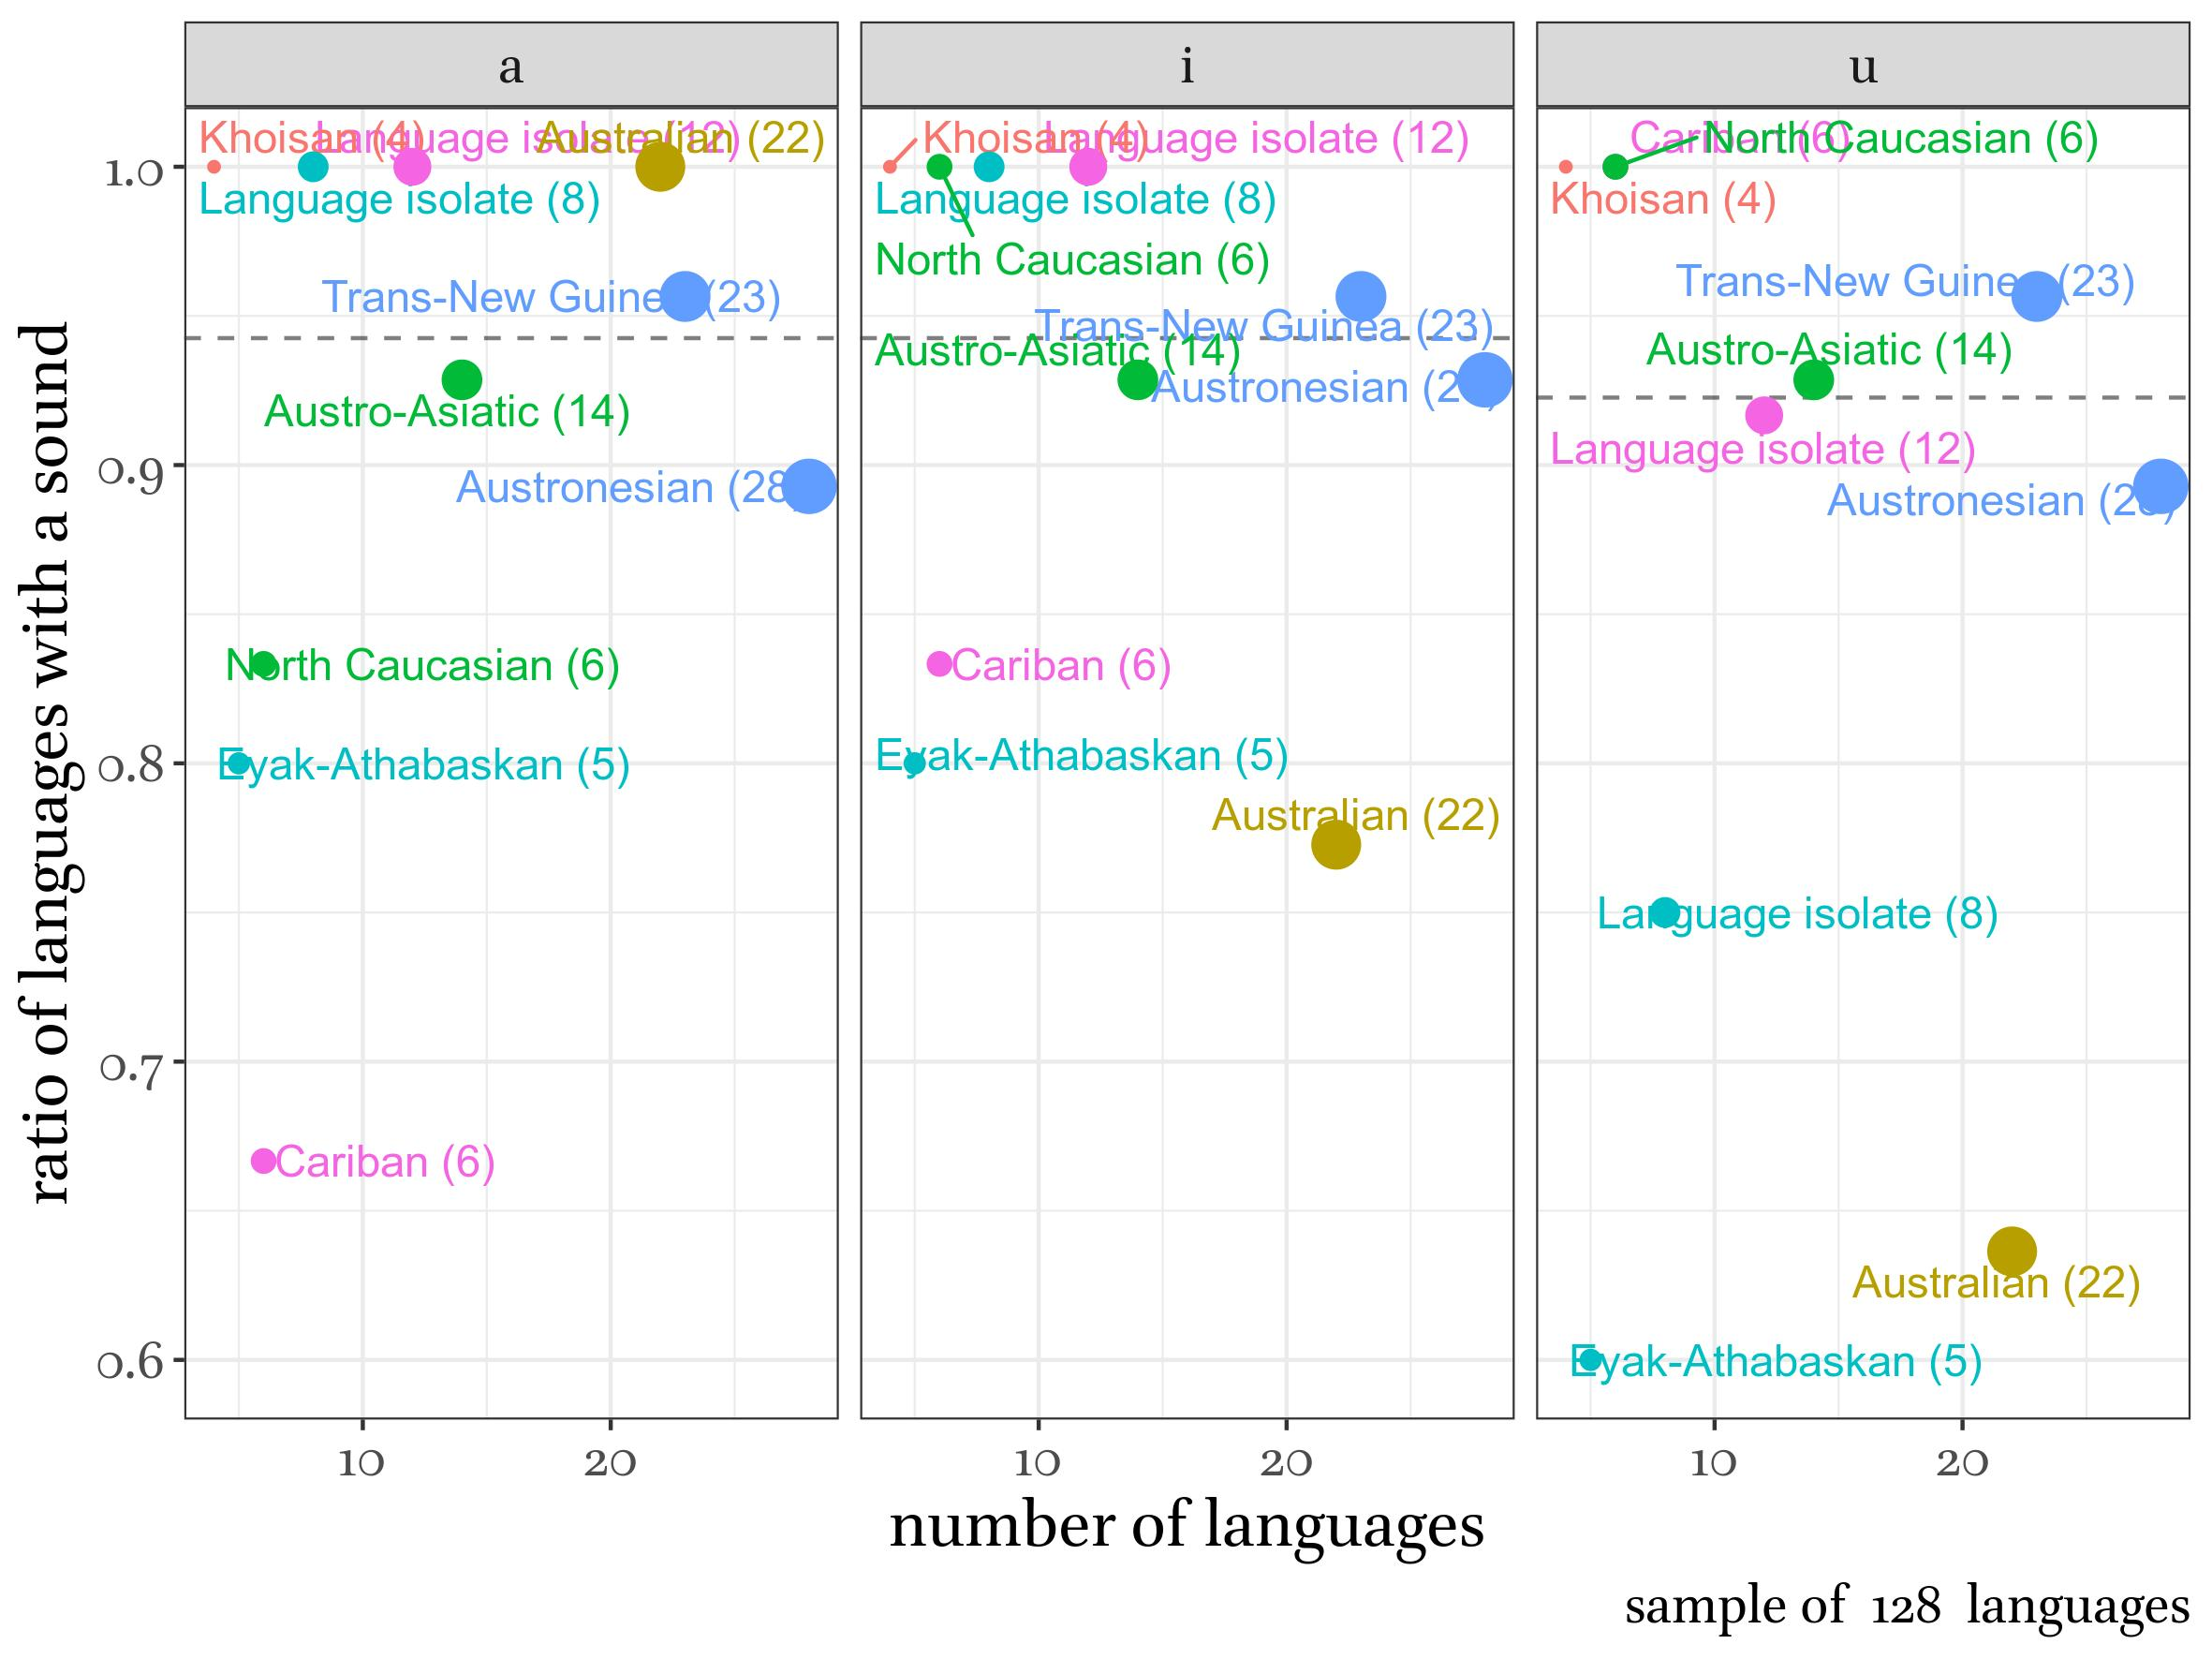
\includegraphics[width = \linewidth]{images/06_families_sample}
\end{frame}

\begin{frame}{Case study: how friquent are \textit{a}, \textit{i} and \textit{u}? (10 families)}
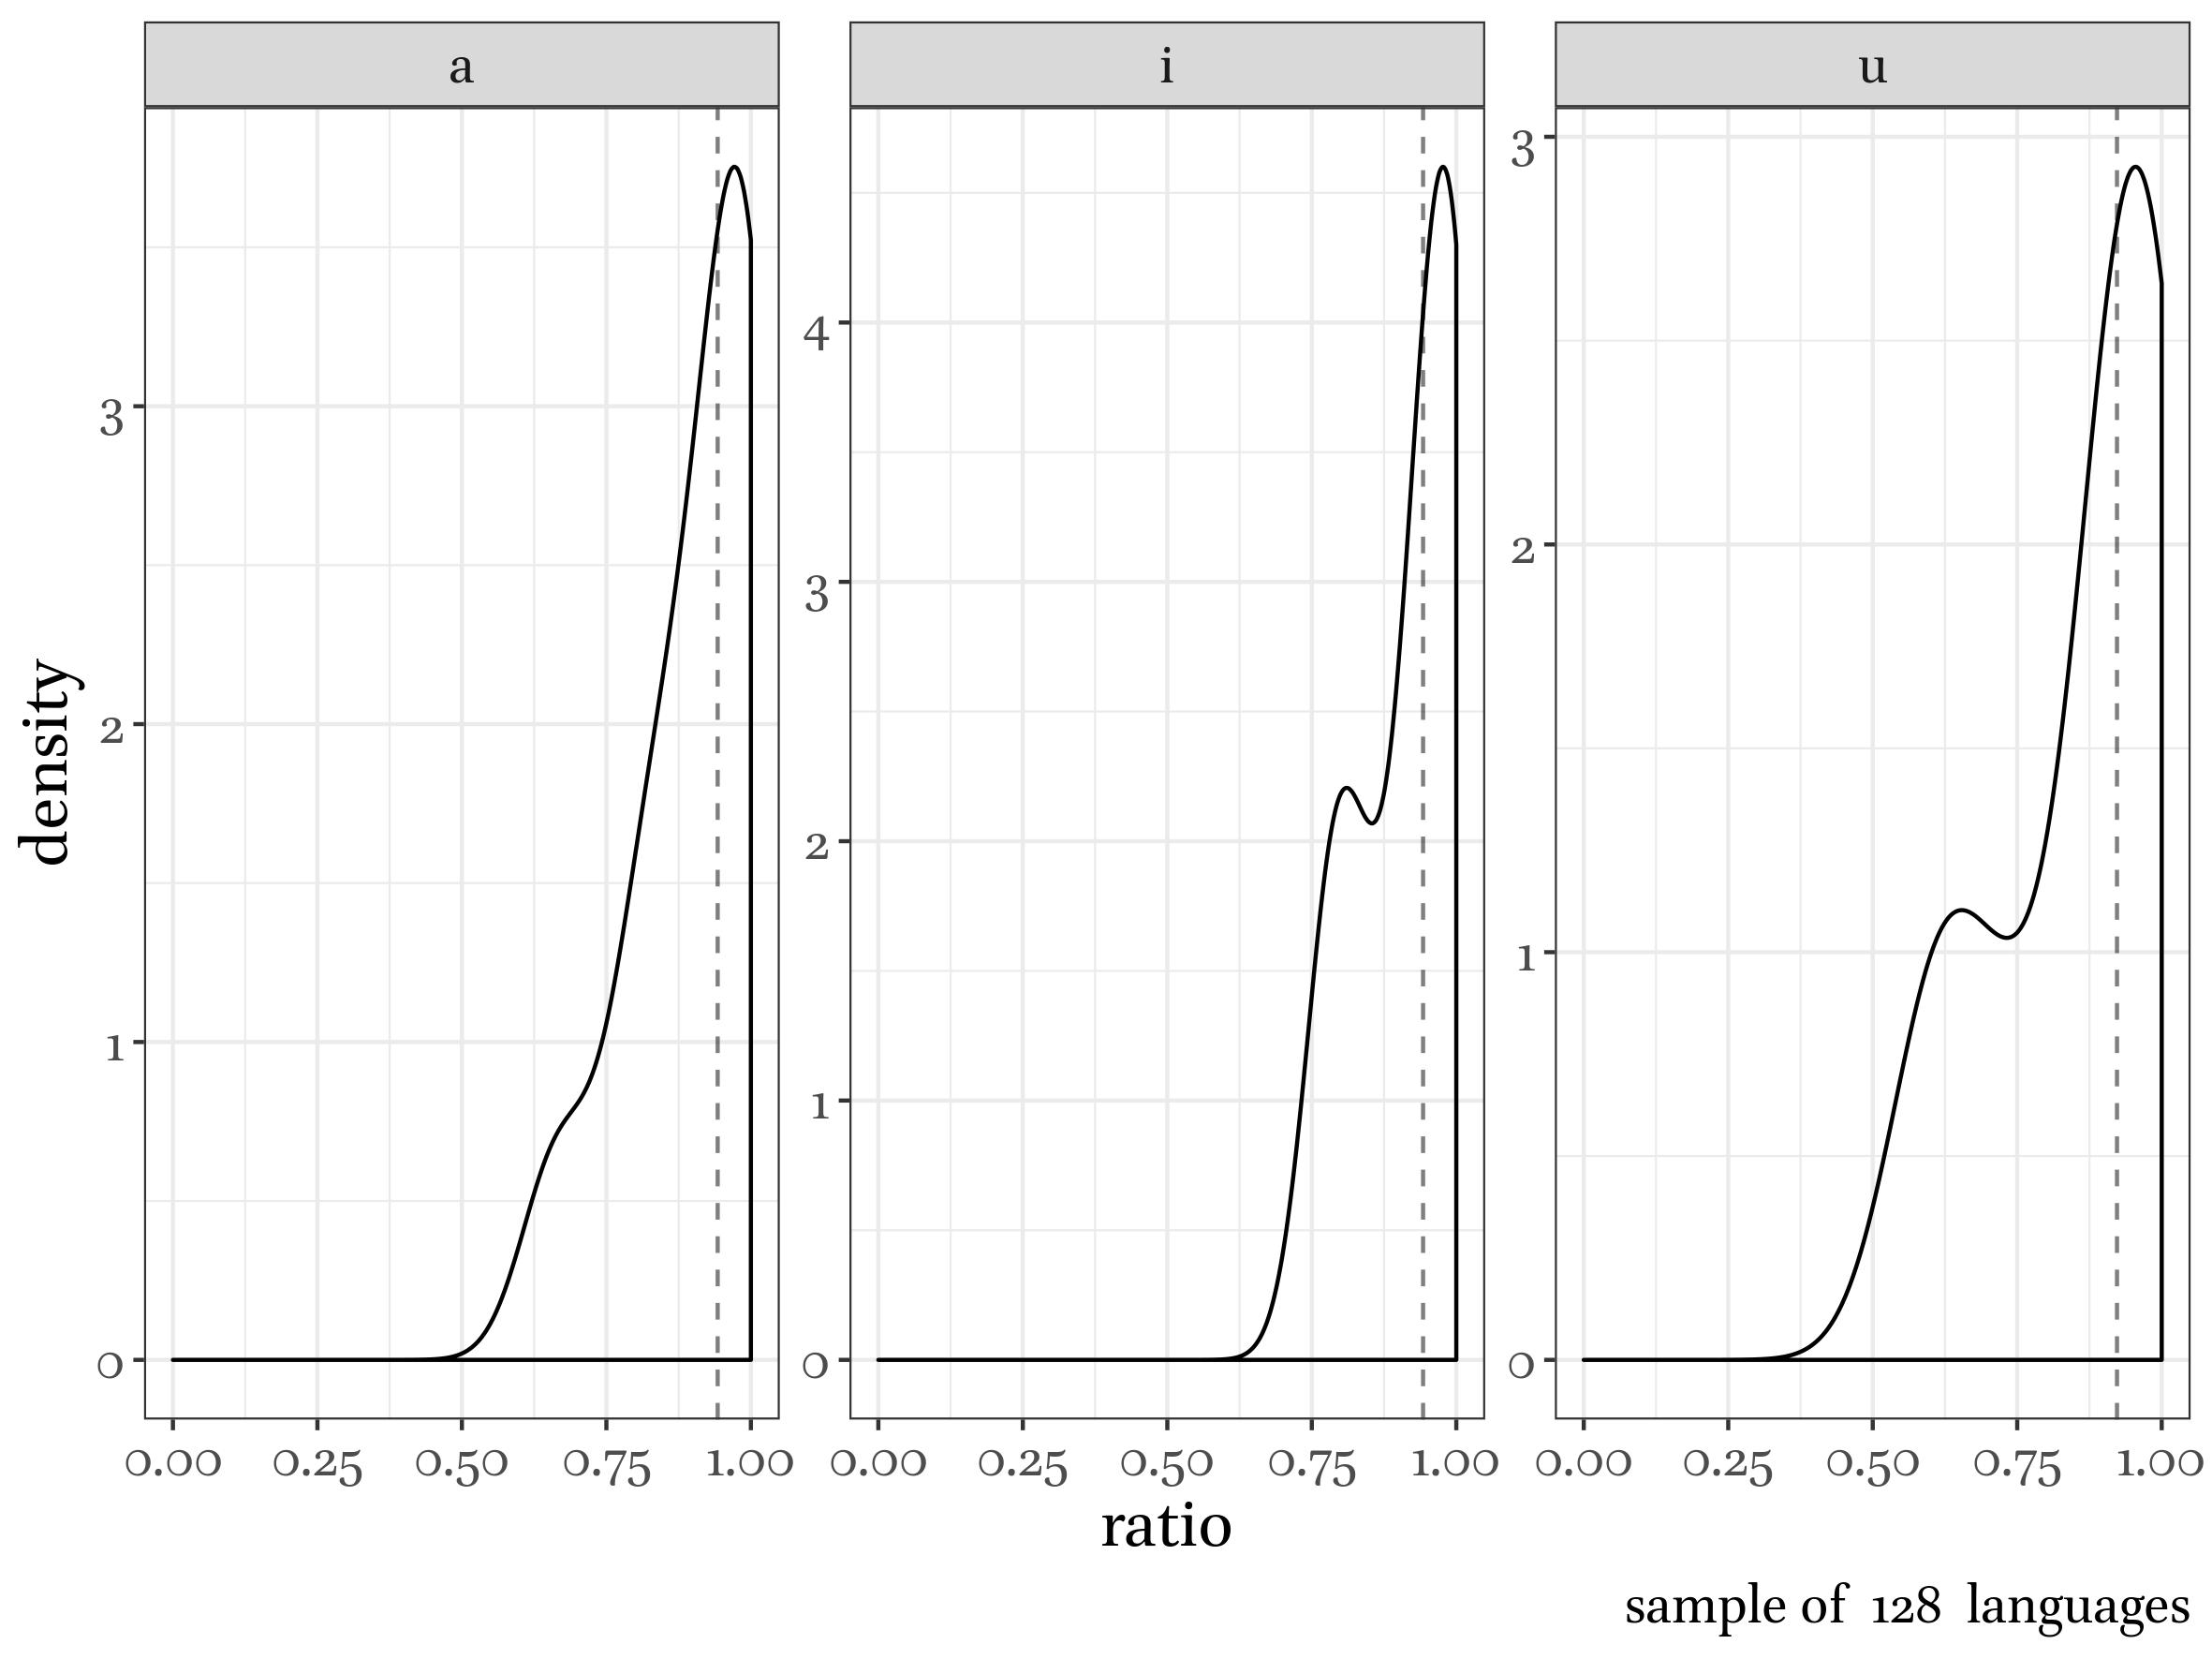
\includegraphics[width = \linewidth]{images/07_distributions}
\end{frame}

\begin{frame}{Case study: how friquent are \textit{a}, \textit{i} and \textit{u}? (29 families)}
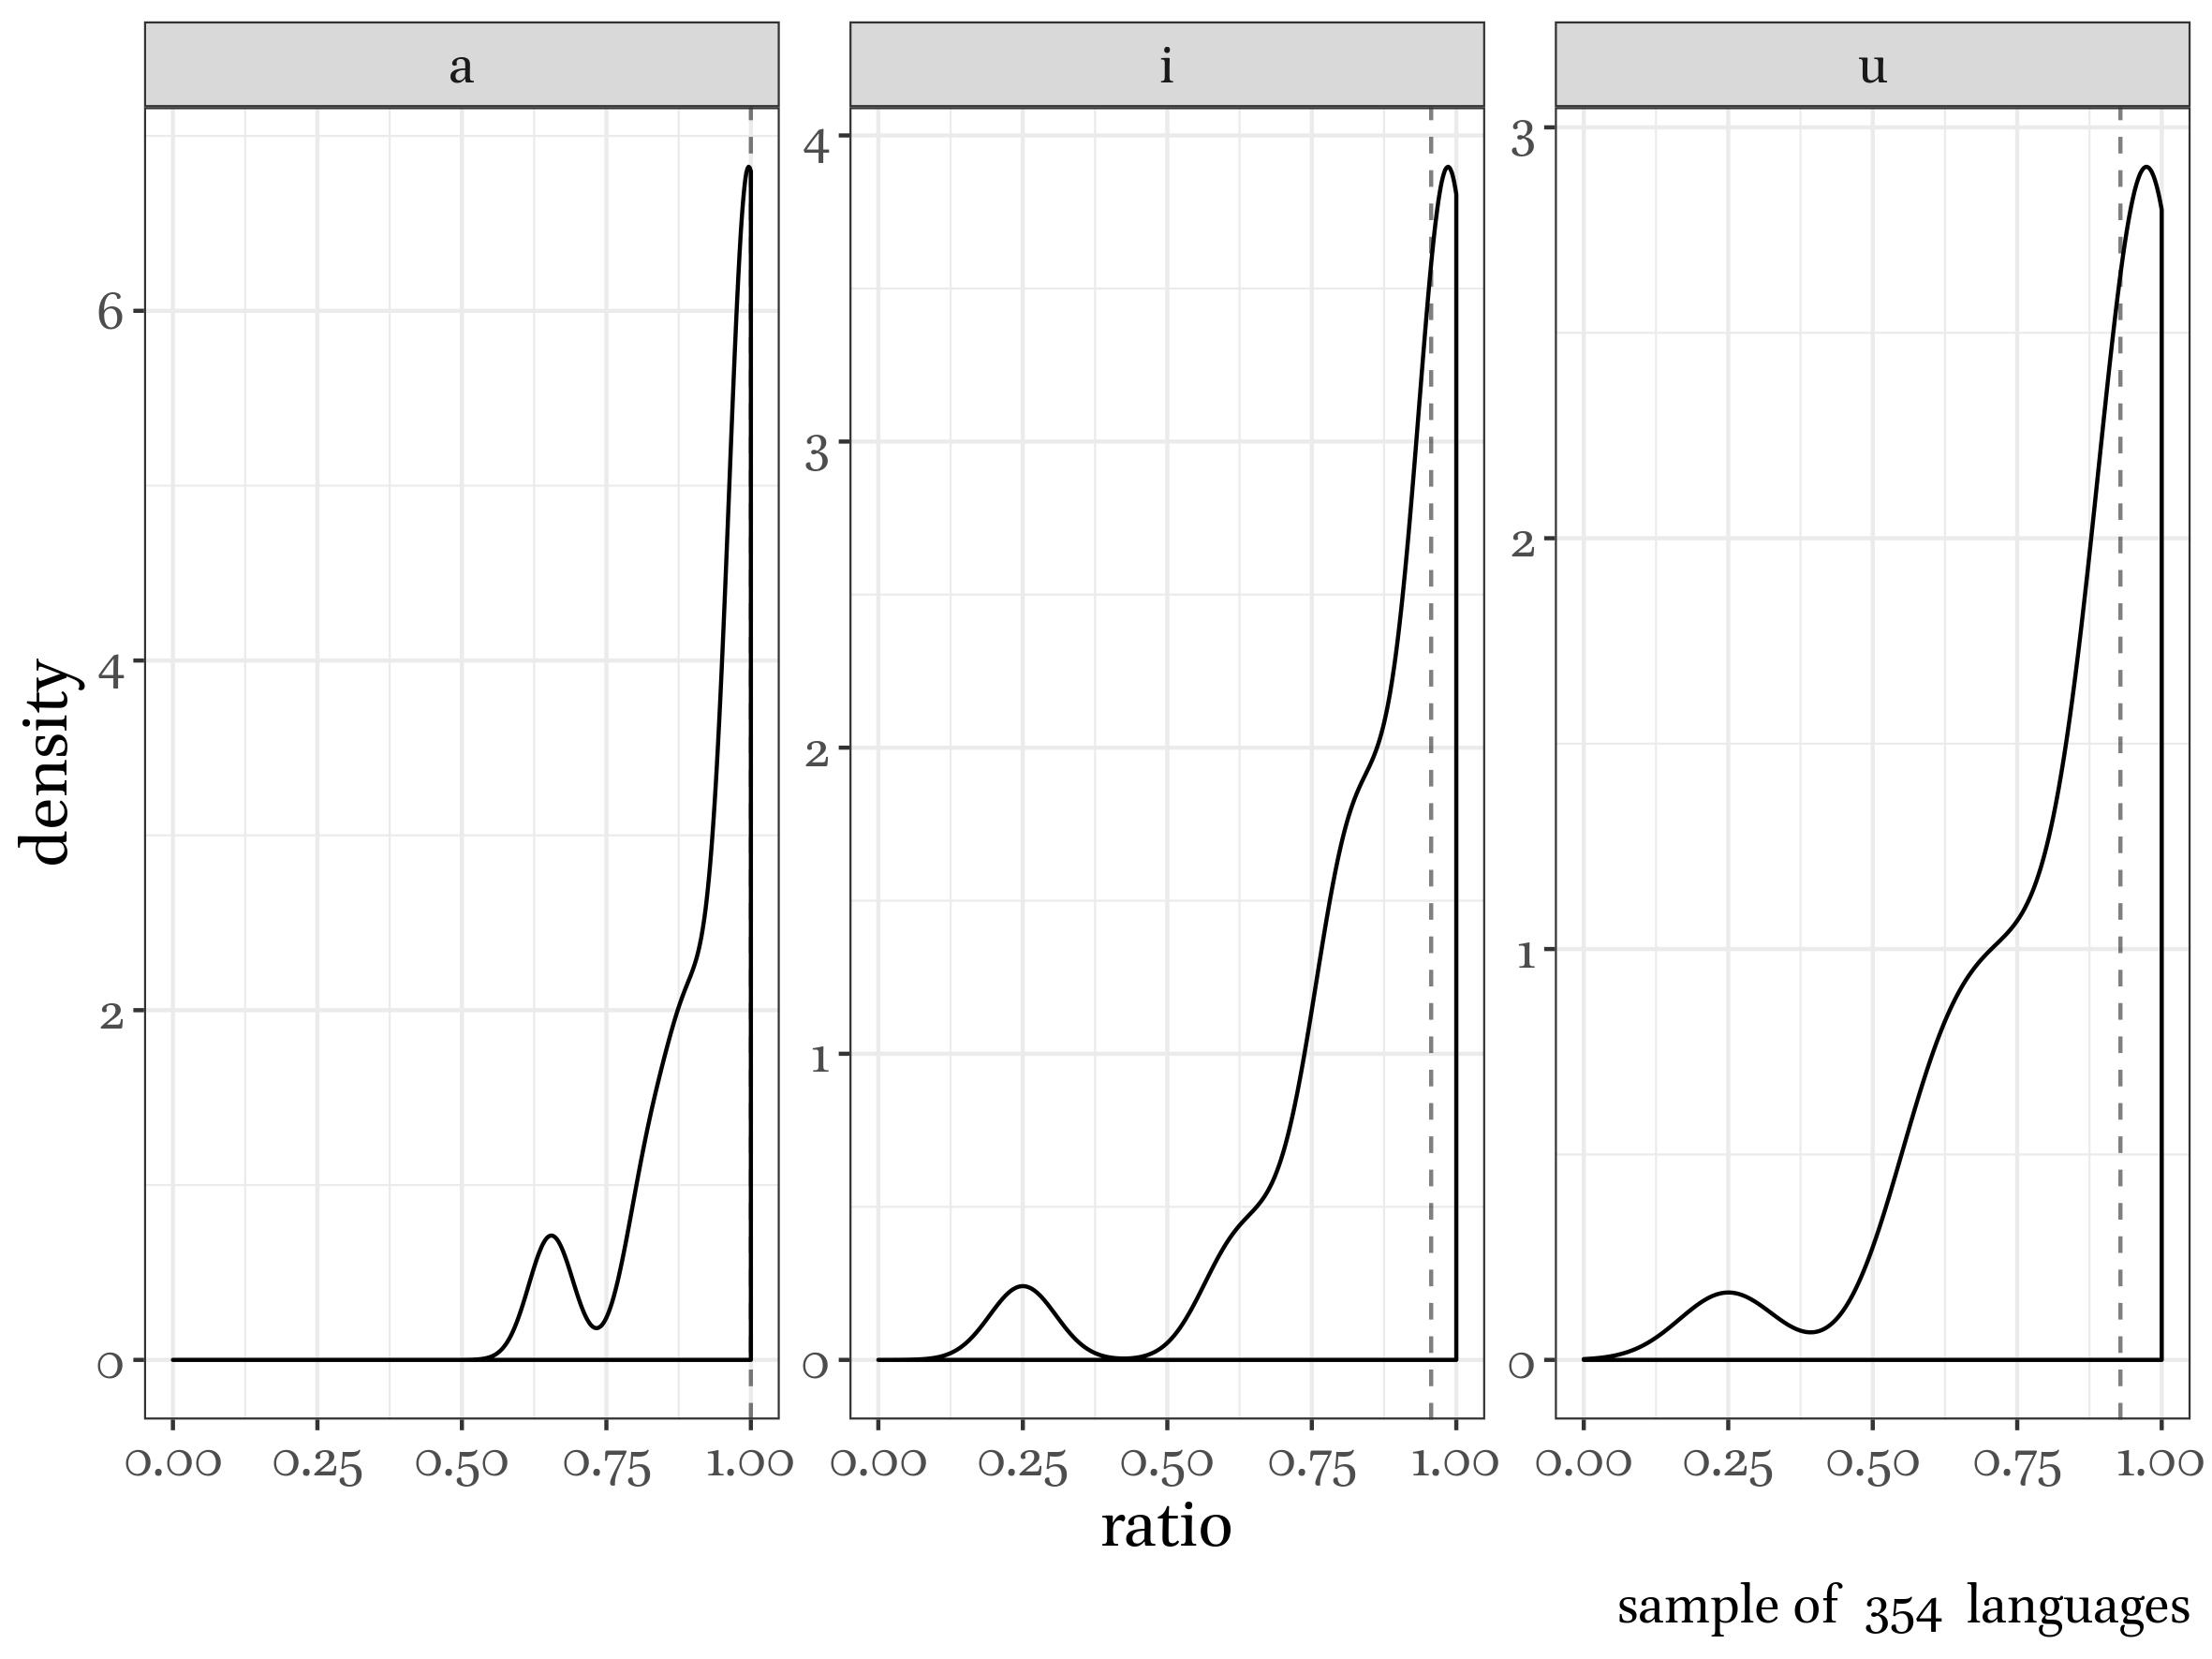
\includegraphics[width = \linewidth]{images/08_distributions}
\end{frame}

\begin{frame}{What about phonology?}
It is possible to use phonological units or relations from any phonological theory you like:
\begin{itemize}
\item Features, feet, syllables, etc.
\item Feature constituents, OT constraints, exemplars, phonological are diachronic alternations
\item Phonological distinctions (e. g. /i/ vs. /ɨ/)
\item ...
\end{itemize}
\end{frame}


\framecard[colorblue]{{\color{colorwhite} \Large Send me a letter!\\
agricolamzgmail.com\\ 
\vfill Presentation is available here: \\tinyurl.com/y3wtkcbq\\
\vfill  
\includegraphics[height = 4cm]{images/02_qrcode}}}

\begin{frame}{References}
\footnotesize
\bibliographystyle{config/chicago}
\bibliography{bibliography}
\end{frame}

\end{document}